%\section{Introducción}
\vspace{1cm}
\itshape
La arquitectura propuesta se centra en la comunicación de la aviónica de un
vehículo espacial, con la característica de que sus componentes (nodos) son
de baja confiabilidad (se piensa en la utilización de componentes COTS)
por lo tanto, es necesario que esta arquitectura sea tolerante a fallas. En este
trabajo el protocolo de comunicación (tolerante a fallas) propuesto,
se encuentra en las capas superiores del modelo de referencia OSI\footnote{ISO/IEC 7498-1 - Open System Interconnection}

Este capítulo está dividido en las seguientes secciones:

\begin{itemize}
\item Arbol de requerimientos, Sección \ref{sec:arbol_req} (página \pageref{sec:arbol_req}).
\item Casos de uso, Sección \ref{sec:caso_uso} (página \pageref{sec:caso_uso}).
\item Diseño estructural (Diagramas de bloques, bloques internos), Sección \ref{sec:dis_estructural}
(página \pageref{sec:dis_estructural}).
\item Diseño dinámico (Diagramas de secuencia, interacción, máquina de estados), Sección
\ref{sec:modelo_dinamico} (página \pageref{sec:modelo_dinamico}).
  
\end{itemize}
\upshape

\noindent\rule{\textwidth}{2pt}

\vspace{1cm}

\section{Árbol de requerimientos}\label{sec:arbol_req}
A continuación se detallan los requerimientos que van a guiar el diseño y
desarrollo de la propuesta de arquitectura de aviónica tolerantes a fallas
basada en componentes \ac{COTS} para satélites. En la Figura
\ref{fig:DiagramaRequerimientos} y en la Tabla \ref{table:Requerimientos} se pueden
observar los requerimientos. 

\begin{figure}[h!]
 \centering
 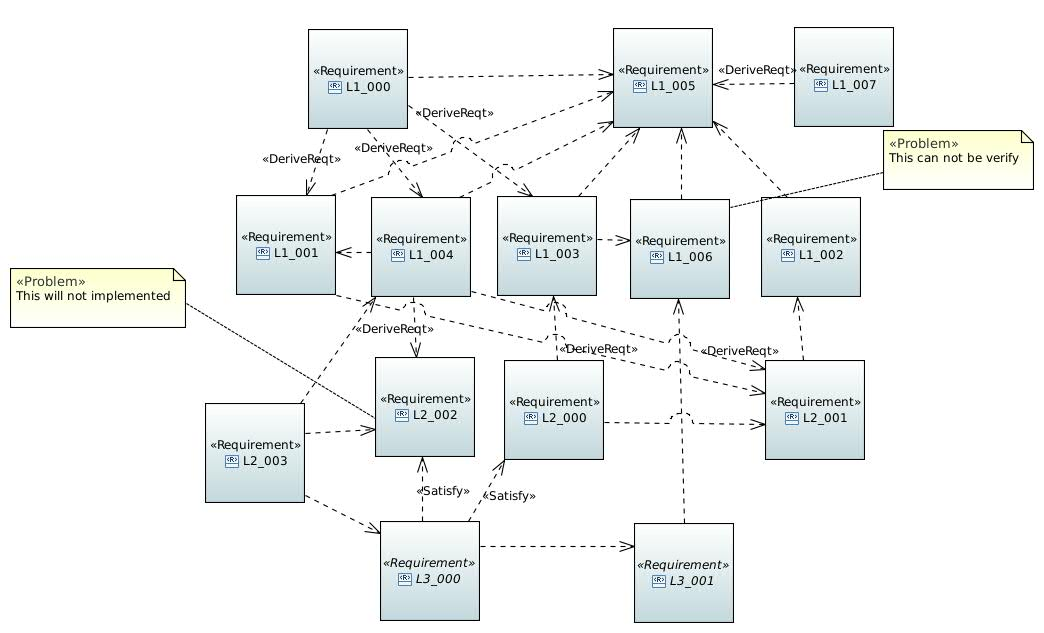
\includegraphics[scale=0.4]{images/Capitulo5/Diagrama_de_Requerimientos.JPG}
  \caption{Diagrama de requerimientos de la arquitectura propuesta}
\label{fig:DiagramaRequerimientos}
\end{figure} 

% \begin{sidewaystable}[]
\begin{table}[]
\small
\centering
\caption{Tabla de Requerimientos}
\label{table:Requerimientos}
%\resizebox{\textwidth}{!}{%
\begin{tabular}{|l|l|l|p{7cm}|p{2cm}|}
\hline
\multicolumn{1}{|c|}{\textbf{}} & \multicolumn{1}{c|}{\textbf{ID}} & \multicolumn{1}{c|}{\textbf{Name}} & \multicolumn{1}{c|}{\textbf{Detail}} & \multicolumn{1}{c|}{\textbf{Kind of Requirements}} \\ \hline
0 & L1\_001 & L1\_001 & The architecture components shall be Commercial Off-The-Shelf category & Constraint \\ \hline
1 & L2\_000 & L2\_000 & The architecture shall be reconfigurate when a node fail. & Funcional \\ \hline
2 & L2\_001 & L2\_001 & Each subsystem shall represented for a Components Off-The-Shelf & Constraint \\ \hline
3 & L1\_000 & L1\_000 & Shall be develop an avionics architecture for spacecraft using Components Off-The-Shelf & Constraint \\ \hline
4 & L1\_002 & L1\_002 & The architecture shall have at least 6 subsystems & Constraint \\ \hline
5 & L1\_003 & L1\_003 & The architecture shall have fault tolerance techniques to assurance the mission life & No funcional \\ \hline
6 & L1\_004 & L1\_004 & The main bus to interconnect components shall be the Controller Area Network Bus developed for Bosch & Constraint \\ \hline
7 & L1\_005 & L1\_005 & The architecture shall be sufficient to make a master degree thesis & No funcional \\ \hline
8 & L2\_002 & L2\_002 & The architecture shall implements a based Controller Area Netowork protocol to intercommunicate the components & Funcional \\ \hline
9 & L3\_000 & L3\_000 & The intercomunication between nodes shall used a Controller Area Netowork protocol based developed in the master degree thesis. & Constraint\\ \hline
10 & L1\_006 & L1\_006 & The architecture shall assurance at least 10 years mission life & No funcional \\ \hline
11 & L3\_001 & L3\_001 & The architecture shall use the distributed network philosophy & Constraint \\ \hline
12 & L1\_007 & L1\_007 & The thesis shall be finished in 1 year & Constraint \\ \hline
13 & L2\_003 & L2\_003 & The nodes shall send and receive message from any nodes connected to the architecture. & Funcional \\ \hline
\end{tabular}%
%}
\end{table}
% \end{sidewaystable}

A continuación se explica cada uno de los requerimientos:
\begin{itemize}
\item\textbf{L1\_000}: Este es el objetivo principal de la presente tesis:
  desarrollar una arquitectura de aviónica tolerante a fallas basada en
  componentes COTS para vehículos espaciales.
\item\textbf{L1\_001}: El principal requerimiento de este trabajo de tesis,
  es desarrollar una arquitectura basada en componentes COTS, lo cual agrega un
  grado importante de innovación tecnológica y complejidad, siendo de especial
  interés para INVAP trabajar con estos tipos de componentes.
\item\textbf{L1\_002}: Este requerimiento hace referencia a que se debe asegurar
  el correcto funcionamiento de la arquitectura con una cantidad de al menos
  6 subsistemas.
\item\textbf{L1\_003}: Este requerimiento exige que la arquitectura sea
  tolerante a fallas para así poder satifacer el requerimiento \textbf{L1\_006}.
\item\textbf{L1\_004}: Este requerimiento (constraint) indica que se debe pensar
  la arquitectura para ser utilizada con el bus CAN de Bosch. Este requerimiento
  es de interés para INVAP.
\item\textbf{L1\_005}: Este requerimiento indica que la arquitectura que se
  desarrolle debe ser suficiente para lograr terminar una tesis de maestría. Por
  el diseño y desarrollo debe ser solo el suficiente y necesario para cumplir
  con el presente trabajo.
\item\textbf{L1\_006}: Este requerimiento indica que debe asegurarse que la
  arquitectura sea lo suficientemente robusta como para asegurar el tiempo de
  vida de la misión de 10 años como mínimo. Existe un \textbf{problema} con este
  requerimiento, y es que para los alcances de esta tesis, será imposible
  verificar si se cumple con este requerimiento.
\item\textbf{L1\_007}: Este requerimiento indica que el trabajo de tesis tiene
  que ser finalizado en menos de un año. Esto tiene relación con el
  requerimiento \textbf{L1\_005} debido a que no se alcanzará el detalle
  necesario para lograr la correcta implementación, verificación y validación de
  la arquitectura.
\item\textbf{L2\_000}: Este requerimiento exige que la arquitectura pueda
  reconfigurarse cuando un nodo falle.
\item\textbf{L2\_001}: Este requerimiento indica que para esta instancia de
  trabajo cada subsistema será tratado como un nodo dentro de la arquitectura.
\item\textbf{L2\_002}: Este requerimiento indica que se debe utilizar dentro de
  la arquitectura un protocolo de comunicación basado en el Bus CAN de Bosch.
\item\textbf{L2\_003}: Este requerimiento asegura que los nodos deben poder enviar
  y recibir mensajes de cualquier otro nodo conectado a la red CANae.
\item\textbf{L3\_000}: Este requerimiento indica que el protocolo de
  comunicación utilizado en esta arquitectura debe estar basado en el
  el protocolo CAN. Este protocolo fue desarrollado en el presente
  trabajo de tesis bajo el nombre de CANae 0.1 Alpha (Vease: Apéndice \ref{Appendix:A}).
\item\textbf{L3\_001}: Este requerimiento exige la utilización de una
  filosofía de red distribuída para su diseño y desarrollo.
\end{itemize}

\section{Casos de Uso}\label{sec:caso_uso}
A continuación se muestra el diagrama de Casos de Uso para la arquitectura propuesta.
El diagrama de Casos de Uso tiene como propósito explicar de manera general
el comportamiento a nivel de sistema de la arquitectura propuesta.
Los actores identificados para esta arquitectura son los diferentes
subsistemas que se conectan a la red a través de los nodos.
Los subsistemas interactúan con el nodo a través de
la aplicación de usuario, es decir, se encuentran asociados.
Se puede observar en la Figura \ref{fig:DiagramaCUArqPropuestaGENERAL}
que de forma general existen tres casos de usos que comprenden el comportamiento
general de la arquitectura. Se tiene \textit{Enviar mensaje} y \textit{Recibir
  Mensaje} los cuales son básicos para cualquier arquitectura de comunicación. A
esto se le agrega el caso de uso de \textit{FDIR} que es el agregado que se le
hace en este trabajo de tesis a través del protocolo de comunicación desarrollado
denominado CANae (Ver apéndice \ref{Appendix:A}). Debe aclararse que en 
la Figura \ref{fig:DiagramaCUArqPropuestaGENERAL}
aparece un resumen de los Actores interactuando con el sistema. 

\begin{figure}[h!]
 \centering
 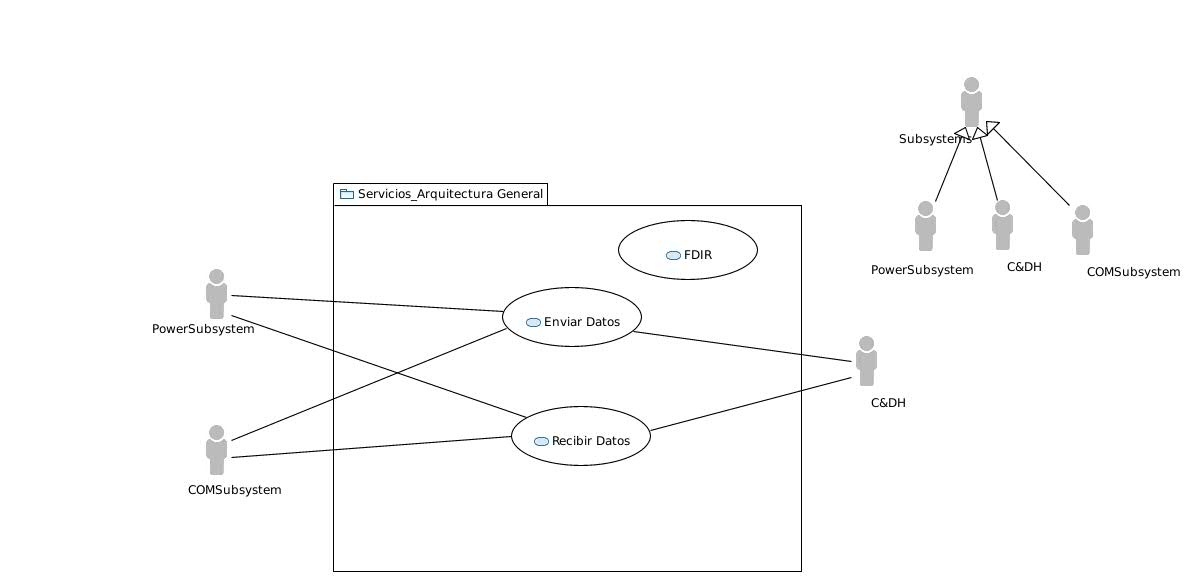
\includegraphics[scale=0.4]{images/Capitulo5/Arq_General.JPG}
  \caption{Diagrama de Casos de Uso General de la arquitectura Propuesta}
\label{fig:DiagramaCUArqPropuestaGENERAL}
\end{figure} 

De manera más detallada en la Figura \ref{fig:DiagramaCUArqPropuesta} se
observa un diagrama de casos de uso explayado que muestra su comportamiento.

\begin{figure}[h!]
 \centering
 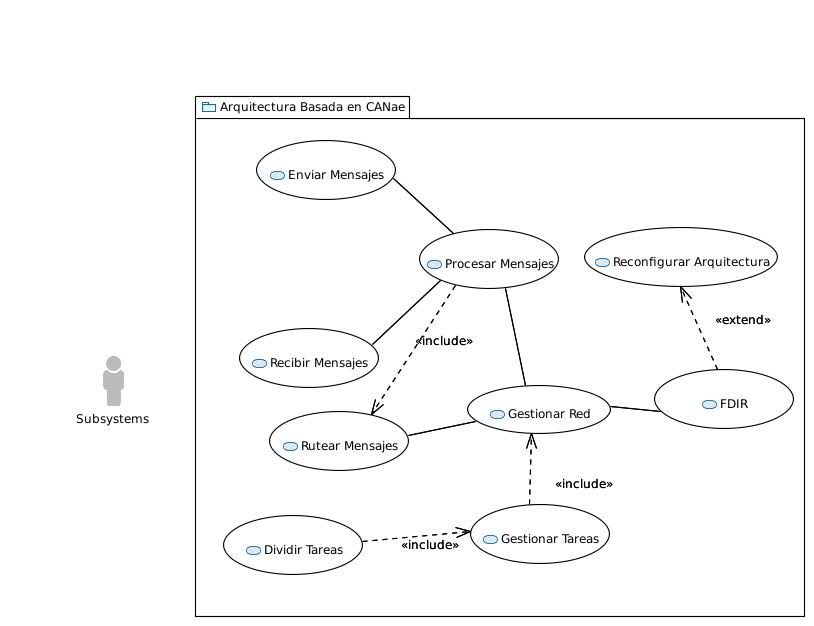
\includegraphics[scale=0.6]{images/Capitulo5/Caso_de_Uso_Arquitectura.JPG}
  \caption{Diagrama de Casos de Uso de arquitectura propuesta}
\label{fig:DiagramaCUArqPropuesta}
\end{figure} 

Le especifcación de los casos de usos se describen en el apéndice \ref{Appendix:UseCase}.
Como se verifica en la Figura \ref{fig:DiagramaCUArqPropuesta}
el sistema tiene 9 casos de uso.

Los casos de uso de \textit{Enviar Mensaje} y \textit{Recibir Mensaje} denota la
capacidad de la arquitectura de enviar y recibir mensajes (Data Frames de
CANae) desde y hacia las aplicaciones de usuario. Cuando una aplicación
necesita enviar un mensaje, estos deben, primero pasar por el caso de uso
\textit{Procesar Mensaje}, debido a que  este es el encargado de empaquetar los mensajes.
También en este punto se encuentra el caso de uso \textit{Rutear
  Mensaje}.

El caso de uso \textit{Rutear Mensaje} se encarga de aplicar los algoritmos
necesarios para lograr entregar el mensaje de una manera eficiente, siguiendo
la tabla de ruteo del CANae. Para esto se basa del caso de uso \textit{Gestionar
  Red}.

El caso de uso \textit{Gestionar Tareas} y \textit{Dividir Tareas} se encarga de
de conocer (periódicamente) el estado de la red y de sus nodos. Con esto, se puede
decidir cómo se reparten las tareas de una manera eficiente, siguiendo
la filosofía de arquitectura distribuída.

Por último tenemos el caso de uso \textit{FDIR} que hace referencia a la
Detección, Aislación, y Recuperación del sistema ante fallas. Debido a la
complejidad de esto, no se desarrolla este caso de uso en la presente tesis.
El cual queda para \textbf{trabajos futuros} \ref{chap:TrabajosFuturos}. En este
caso de uso se encuentra el \textit{Reconfigurar Arquitectura}. Este es un
algoritmo del \ac{FDIR} que cuando se produce una falla en algunos de los
nodos, la red se tiene que reconfigurar, para lograr continuar funcionando,
aún cuando haya nodos inactivos. Esto le brindaría a la arquitectura una grado
más de tolerancia a fallas. 

% talk about structural design
\section{Diseño Estructural}
gil


% talk about behavorial design
\section{Modelo dinámico}\label{sec:modelo_dinamico}
En esta sección se modelará el comportamiento de la arquitectura.
A diferencia de lo modelos  que se estudió en la sección anterior (diagramas
de bloques, diagrama de bloques internos) que hacen referencia al
\textit{qué} del sistema, en el modelado del comportamiento se
hace referencia al \textit{cómo} del sistema. Este \textit{cómo}
es descripto por el modelado del comportamiento dentro del
sistema \citep{HoltPery}.

En esta sección se verán  3 diferentes niveles de abstracción
de los modelos de comportamiento del sistema. En primer lugar, el
nivel más alto de abstracción es la máquina de estado, que considera la
interacción entre bloques. El siguiente diagrama que se verá es
el diagrama de secuencia, el cual pone en manifiesto los diferentes
mensajes que son enviadas entre las entidades. Y por último, se
desarrolla el diagrama de actividades, siendo este el nivel
más bajo de abstracción del modelado del comportamiento del sistema.

\subsection{Máquina de estado}
En esta subsección se describe el ciclo de vida de los
bloques que conforman la arquitectura. En resúmen, lo que se
pretende demostrar, es el comportamiento de los objetos de la
arquitectura.

En la Figura \ref{fig:StateMachineArqCompleta} se presenta la
máquina de estado de la arquitectura completa.  En esta se
puede observar todos los estados por los cuales la arquitectura
debe recorrer.

\begin{figure}[h!]
 \centering
 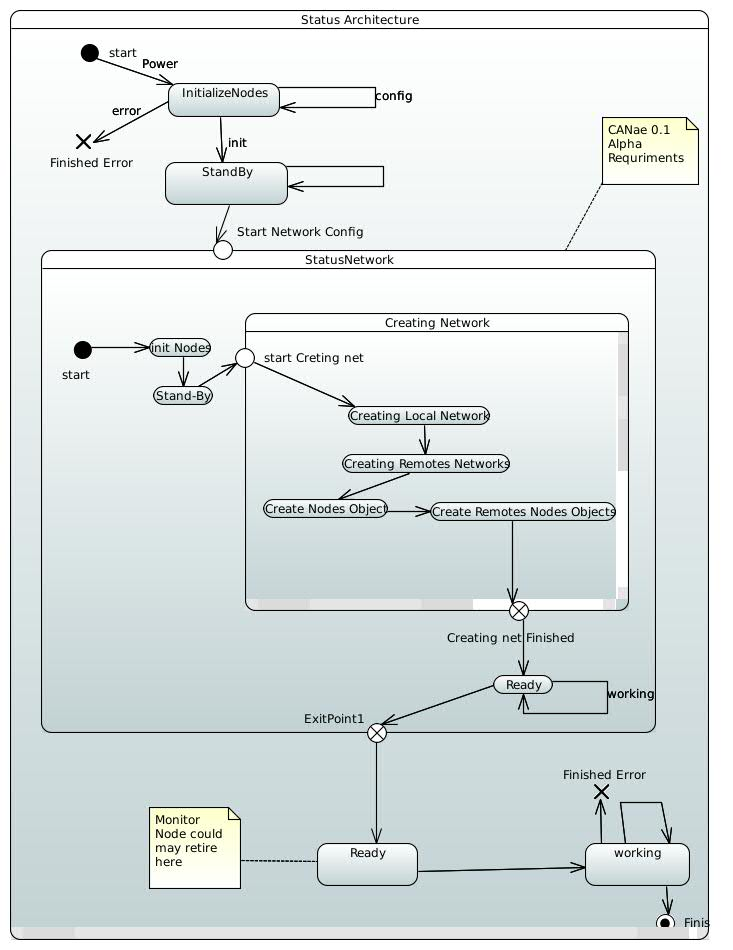
\includegraphics[scale=0.4]{images/Capitulo5/StateMachineArqCompleta.JPG}
  \caption{Máquina de estado de la arquitectura completa}
\label{fig:StateMachineArqCompleta}
\end{figure}

A continuación se procede a explicar la máquina de estado. Todo
inicia en el momento en el que la red es alimentada (eléctricamente)
siguiendo los protocolos de CAN \citep{can-ciaWEB}. En primer lugar, la
red pasa a un estdo de inicialización de los nodos, en los cuales, estos
son alimentados, se encienden, y comienzan con todos los procedimientos
normales de cualquier sistema embebido. Los cuales son Booteo, checkeo del
funcionamiento y del estado de salud del propio \ac{HW} y los \ac{HW}
conectados a él. Esto incluye la iniciación, del protocolo CANae como
un stack más del servicio del sistema operativo o sistema embebido
que gobierna a cada uno de los nodos. Esto se observa en la Figura
\ref{fig:StateMacineInitNodes}.

\begin{figure}[h!]
 \centering
 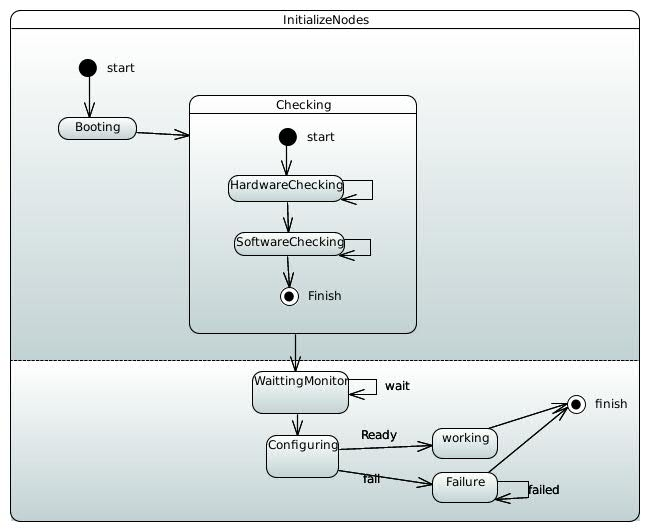
\includegraphics[scale=0.4]{images/Capitulo5/InitializeNodes.JPG}
  \caption{Máquina de estado de los nodos.}
\label{fig:StateMacineInitNodes}
\end{figure}

Una vez que todos los nodos se encuentran inicializados, y la red se encuentra
estable\footnote{Defínase como estable, la situación en la que el
  protocolo CANae se inicializó correctamente y está listo para pasar
  a la segunda etapa.}, la arquitectra pasa a un estado de Stand-By.
En este estado, la arquitectura espera por la orden del nodo monitor
para comenzar a configurar la red. Aquí se sigue lo indicado en el
protocolo CANae (Véase apéndice \ref{Appendix:A}). En primer lugar,
se crean las instancias de red localmente. Luego,  el nodo monitor
coordina la creación de las instancias de red remota. Luego se crean
los objetos nodos tanto locales como remotos. Estas actividades
son necesarias para lograr establecer una correcta comunicación
entre nodos utilizando el protocolo CANae (Versión 0.1 Alpha).

Una vez finalizada la creación de la red, la arquitectura completa
pasa a un estado Ready, donde el nodo monitor ya puede ser retirado.
Luego, la arquitectura ignora el nodo monitor (Si todavía se encuentra
conectado) y ya puede comenzar a trabajar normalmente.

\subsection{Diagrama de secuencia}
A continuación se muestra los diagramas de secuencias, para entender
cuál es el comportamiento de la arquitectura, en un grado
de abstracción menor.

En la Figura \ref{fig:SecInitArq} se puede observar como en
el momento de alimentar (eléctricamente) a los nodos, este comienza,
en primer lugar, a ejecutar el boostrap. Este bootea al
sistema operativo (o sistema embebido según sea la tecnología
que se utilice). Una vez que el sistema operativo es cargado se
deben ejecutar (preferentemente) dos tipos diferentes de chequeos:
\begin{itemize}
\item Hardware Check
\item Software Check
\end{itemize}

\begin{figure}[h!]
 \centering
 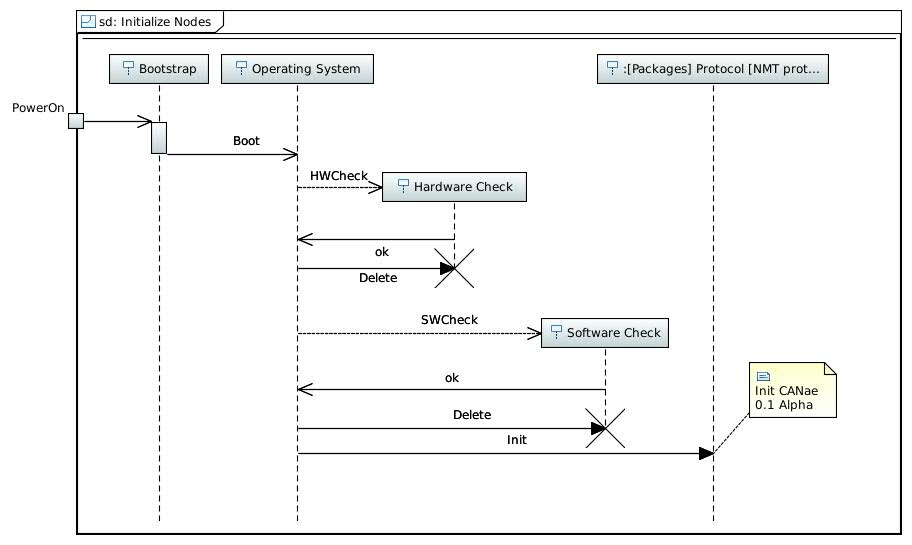
\includegraphics[scale=0.4]{images/Capitulo5/SecuenciaIInitNodes.JPG}
  \caption{Diagrama de secuencia del inicio de la arquitectura.}
\label{fig:SecInitArq}
\end{figure}

Estos son dos piezas de código. El primero tiene como tarea principal
chequear el estado de salud de los equipos de hardware, tanto
del propio nodo, como así también del subsistema que tiene más proximo.
Como se expuso en la subsección \ref{subsec:bridge} cada nodo tiene
próximo a él (físicamente hablando) un subsistema (con su computadora
de vuelo). Por lo tanto el nodo se debe encargar de chequear el
estado de salud de los diferentes componetes de ese subsistema. El
segundo chequeo, se ocupa de verificar el estado de salud del software
tanto del nodo, como del subsistema más próximo.

Luego de que los chequeos se hayan resuelto exitosamente se crea una
instancia del protocolo CANae y da inicio a su servicio NMT. Este
servicio se puede observar en la Figura \ref{fig:NMTC5}. En primer lugar
se debe esperar que el nodo monitor esté inicializado, y este les
envía un mensaje de \textit{crete\_remote\_network()} a todos los
nodos conectados a la arquitectura. Este mensaje llega al NMT del
protocolo de CANae de todos los nodos.

\begin{figure}[h!]
 \centering
 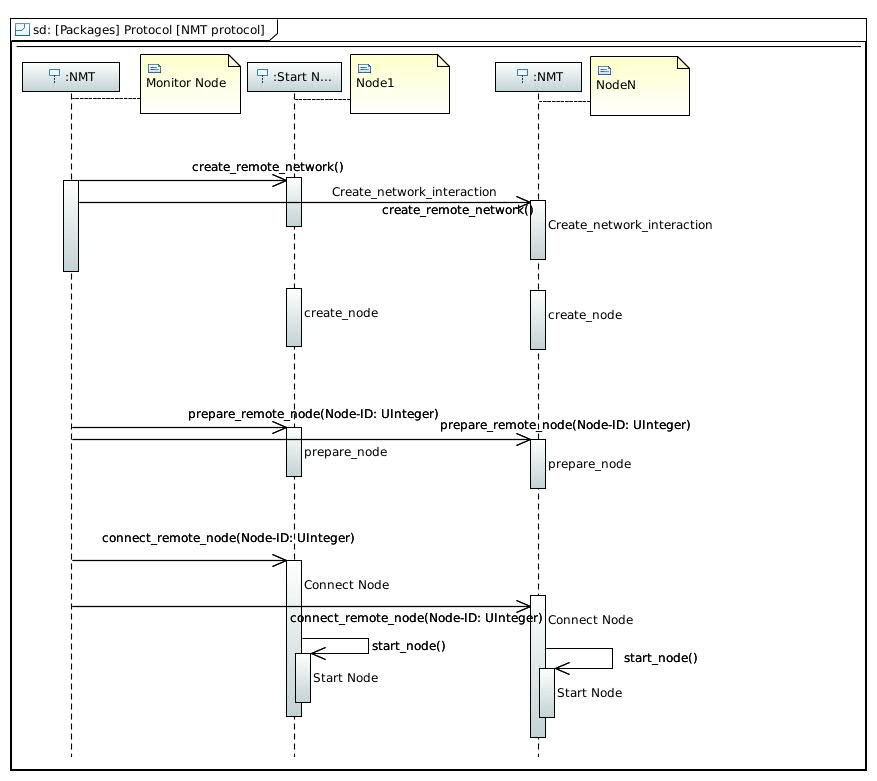
\includegraphics[scale=0.4]{images/Secciones/AppendixA/Protocol_NMT.JPG}
  \caption{Diagrama de secuencia de CA}
\label{fig:NMTC5}
\end{figure}

Luego, siguiendo el protocolo de CANae, cada nodo crea su instancia de
nodo. Esto puede observarse en la Figura \ref{fig:CreateNodeNMTC5}.
El objeto de \textit{CANAppLayerController} envía el mensaje \textit{
  create\_node()} al \textit{NodeManagement} de \textit{create\_newtork\_object()} con el objetivo de crear una instancia local de la red.


\begin{figure}[h!]
 \centering
 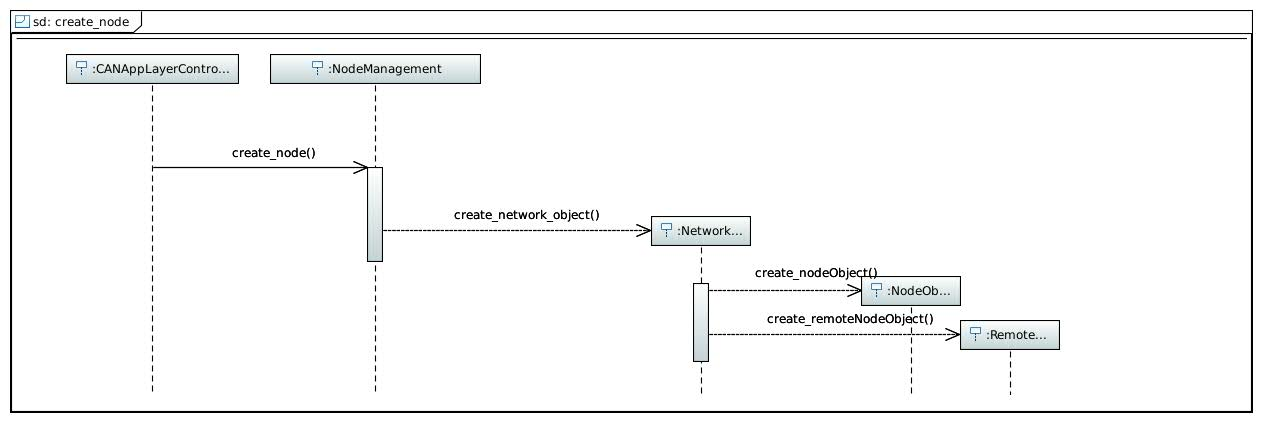
\includegraphics[scale=0.4]{images/Secciones/AppendixA/create_node.JPG}
  \caption{Crear Objecto Red, Objeto Nodo y Objeto Nodo Remoto}
  \label{fig:CreateNodeNMTC5}
\end{figure}

Luego el nodo monitor envía el mensaje \textit{prepare\_remote\_node()}.
El protocolo CANae preve los pasos que se muestran en la Figura
\ref{fig:PrepareNodeC5}

\begin{figure}[h!]
 \centering
 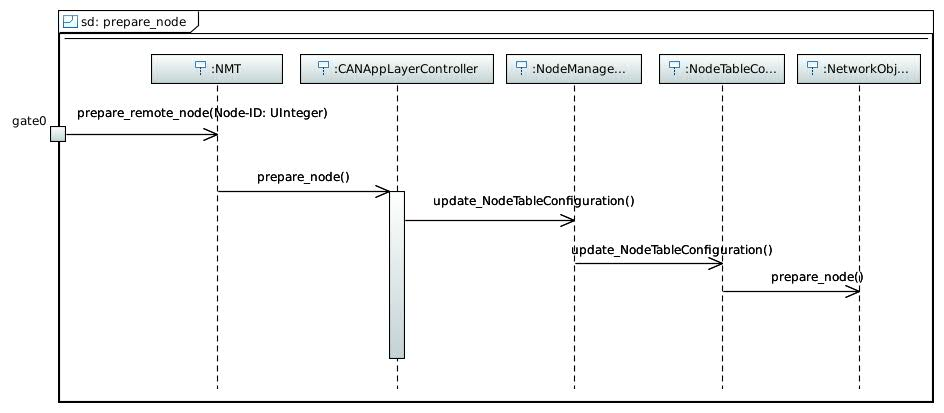
\includegraphics[scale=0.4]{images/Secciones/AppendixA/PrepareNode.JPG}
  \caption{Preparar nodo para la conexión a la red CAN}
  \label{fig:PrepareNodeC5}
\end{figure}

Por último, se conectan todo los nodos a la red, para lo cual deben
actualizar el \textit{Node Table Configuration}, y finalmente ya
pueden comenzar a comunicarse. Esto se observan en las Figuras
\ref{fig:PrepareNodeC5} y \ref{fig:ConnectNodeC5}

\begin{figure}[h!]
 \centering
 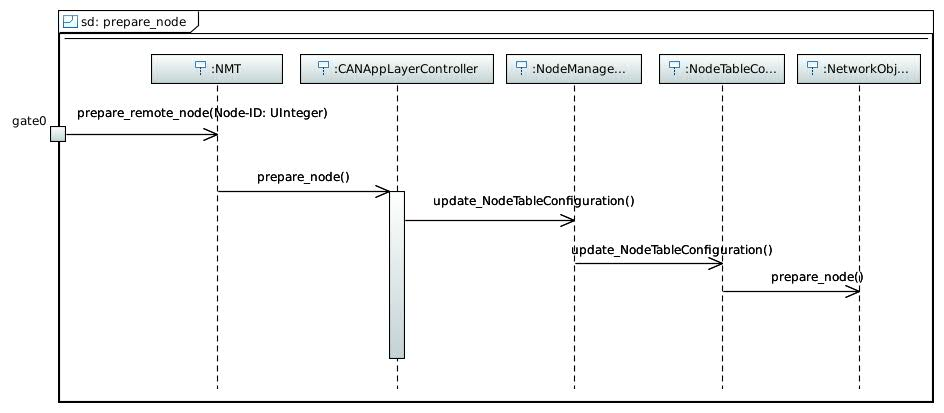
\includegraphics[scale=0.4]{images/Secciones/AppendixA/PrepareNode.JPG}
  \caption{Preparar nodo para la conexión a la red CAN}
  \label{fig:PrepareNodeC5}
\end{figure}

\begin{figure}[h!]
 \centering
 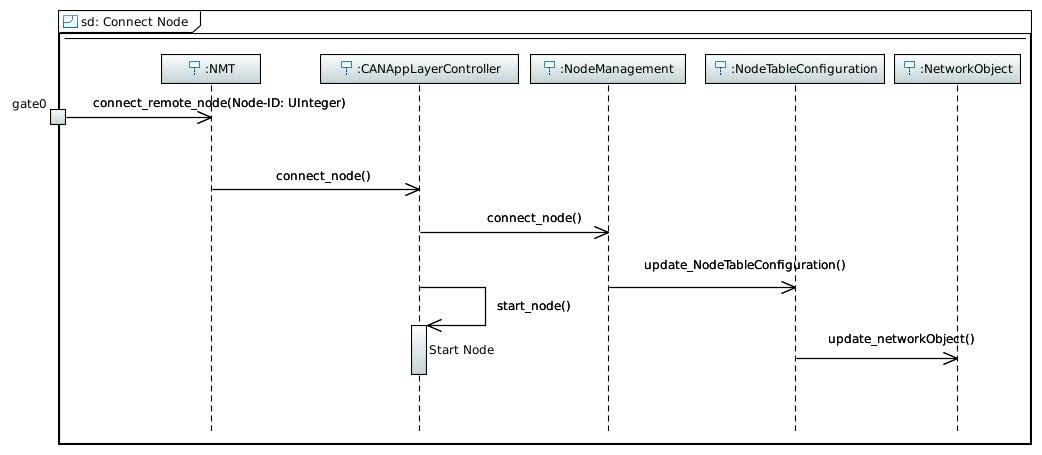
\includegraphics[scale=0.4]{images/Secciones/AppendixA/connect_node.JPG}
  \caption{Conectar el nodo a la red CAN}
  \label{fig:ConnectNodeC5}
\end{figure}

\subsection{Diagrama de actividades}
En esta subsección se verá algunos diagramas de actividad para modelar
el comportamiento de la arquitectura propuesta. Los diagramas de actividades
comúnmente son utilizados, generalmente, para describir el comportamiento
a muy bajo nivel (a nivel de componentes), en otras palabras para modelar
procesos, mientras que los diagramas de secuencia muestran el comportamiento
entre elementos, y las máquinas de estados  muestran el comportamiento
dentro de los elementos \citep{HoltPery}.

En la Figura \ref{fig:initNodes} se puede observar el proceso, en detalle,
del inicio de los nodos. Todo comienza cuando se alimenta (eléctricamente)
el nodo. En primer lugar, se ejecuta (como ocurre normalmente) el bootstrap,
este bootea al sistema operativo o al sistema embebido (dependiendo de como
se implemente). Los siguientes pasos son los esperados para cualquier sistema
espacial. Se chequea el \ac{HW} propio del nodo, se chequea memoria y componentes.
Luego, se chequea el estado de salud del subsistema. Para ello, se puede pedir
el chequeo a la CPU del subsistema, y este a vez, chequea los componentes
propios del subsistema.

Con estos pasos se puede obtener el Houskeeping (HK) tanto de \ac{HW} propio del nodo
como del subsistema. Este HK es recibido por el sistema operativo
(o sistema embebido), y se comienza a hacer un chequeo del lado del
software. Esto significa que se pueden realizar cualquier tipo de actividad
para chequear que las tareas (o procesos) se ejecuten correctamente.

Para finalizar, el sistema operativo crea una instancia del stack de servicio de
comunicación, dónde se encuentra el protocolo de comunicación CANae.

Debe observarse que el chequeo de \ac{HW} tanto propio como el del
subsistema se encuentra dentro de lo que se denomina \textit{zona interrumpible},
esto significa que si se da alguna \textit{Falla} (Failure en la Figura), debe
activarse el sistema FDIR del nodo. Este, lo que busca en primer lugar,
es detectar la falla, dónde se produjo y por qué. Luego, el sistema trata de
aislar la falla para que no afecte a ningún otro componente. Por último, el
sistema hará el intento de recuperarse de la falla, en el caso de que se
recupere correctamente, se regresa la tarea de chequeo, para
llevar a cabo estas actividades nuevamente; en caso contrario se termina la actividad.

\begin{figure}[h!]
 \centering
 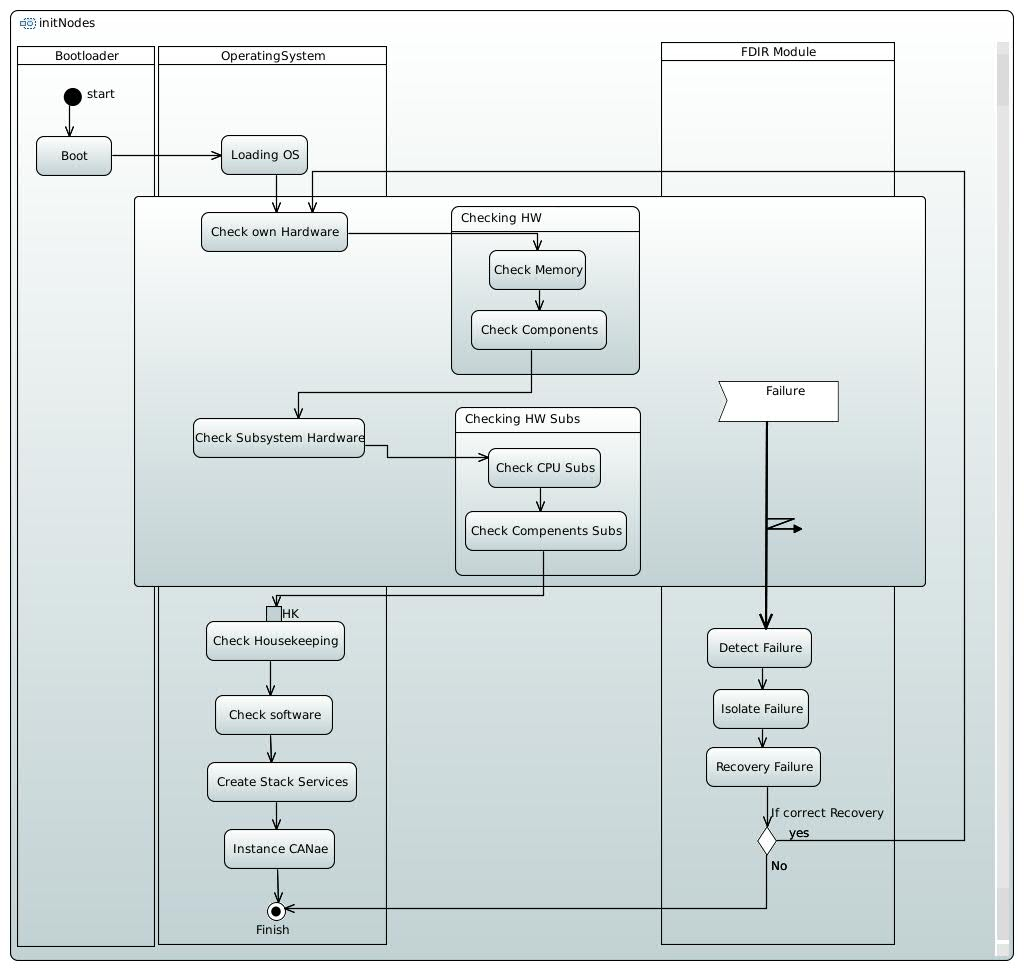
\includegraphics[scale=0.4]{images/Capitulo5/initNodes.JPG}
  \caption{Diagrama de actividades del inicio de nodos}
  \label{fig:initNodes}
\end{figure}

Otra parte importante a modelar de la arquitectura propuesta, es el momento
de la creación de la red CANae. Como se mencionó anteriormente el protocolo
CANae (Véase apéndice \ref{Appendix:A}) requiere de la existencia de un nodo monitor
para coordinar la creación de la red CANae. Este modelo se puede observar
en la Figura \ref{fig:NodeMonitor}.

El nodo monitor inicia la creación y configuración del nodo enviando la
señal \textit{create\_remote\_network()} a todos los nodos conectados a la
red. Cada nodo que recibe la señal, lleva a cabo todas las actividades prevista
por el protocolo CANae para la creación y configuración de la red. Crea las instancias
de la red remota, los objetos red, crea la tabla de configuración de nodos y crea
por último las instancias de los nodos.

\begin{figure}[h!]
 \centering
 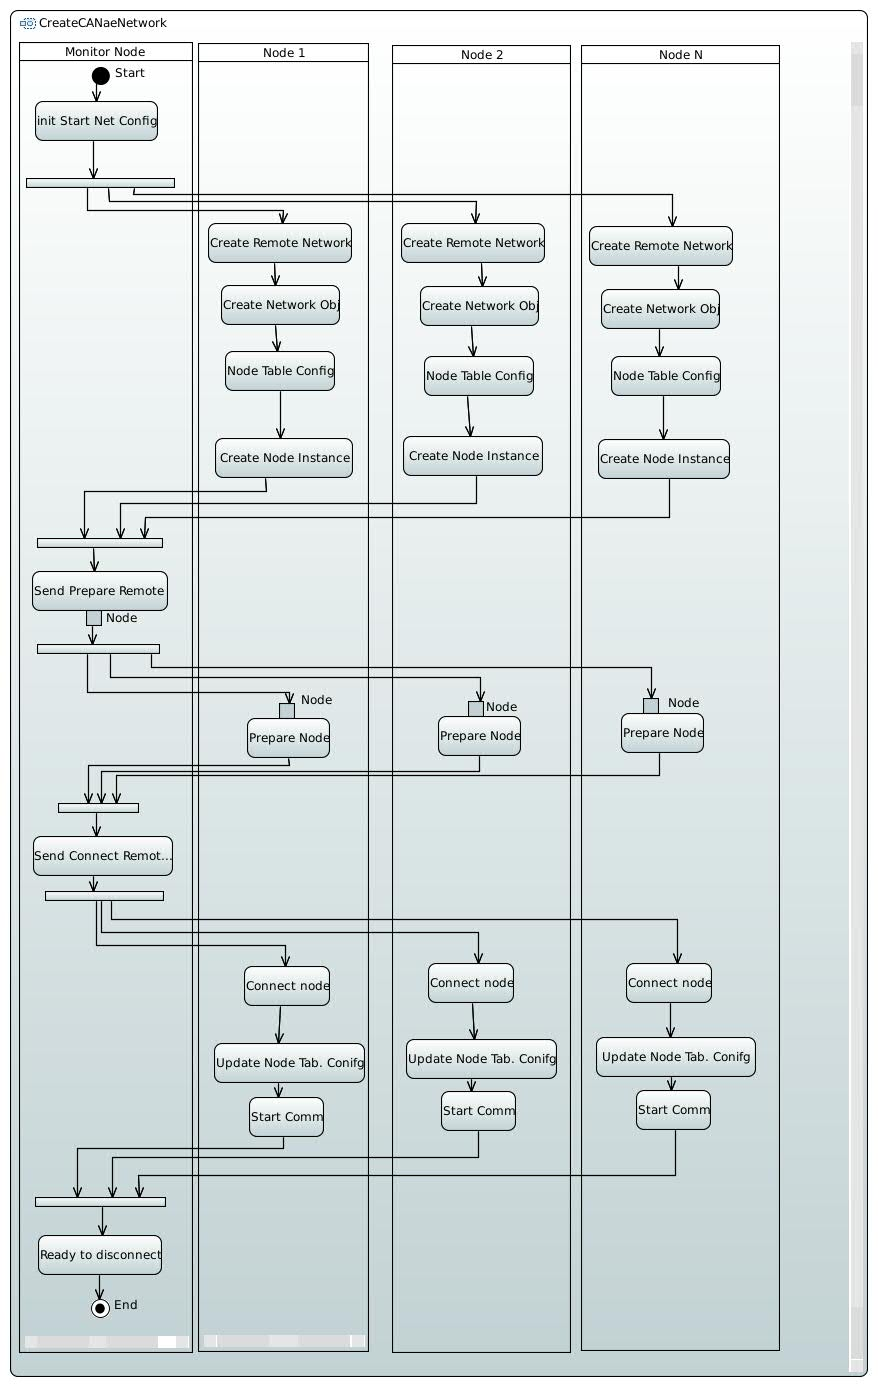
\includegraphics[scale=0.4]{images/Capitulo5/NodeMonitor.JPG}
  \caption{Diagrama de actividades del inicio de nodos}
  \label{fig:NodeMonitor}
\end{figure}

Como segundo paso, el nodo monitor envía la señal de \textit{Prepare Remote Node}, la
cual es recibida por todos los nodos y se preparan internamente para comenzar a
comunicarse.

Por último,  el nodo nodo monitor envía la señal para que los nodos se conecten a
la red. Cada nodo se conecta, y actualiza su tabla de configuración del nodo. A partir
de este momento los nodos ya pueden comenzar a enviar mensajes y el nodo monitor ya
puede ser extraído de la red. 

Además, se modela el ``cómo'' se comporta la arquitectura al
momento de tratar de enviar un mensaje de uno nodo a otro nodo. Esto se puede
observar en la Figura \ref{fig:SendMessage}. En primer lugar el nodo emisor,
debe ``preparar'' el mensaje. Esto significa que debe empaquetarlo para,
cumplir tanto con los protocolos CANae, como así también con el procolo CAN.

Como segundo paso se debe consultar a la tabla de configuación del nodo para conocer
cuál es el camino óptimo para llegar a entregar el mensaje. Para ello se le aplica algún
algoritmo de ruteo.

Por último, se envía el mensaje através del microcontrolador CAN. Este es recibido por el nodo
destino y luego es procesado. Esto puede observarse, con mayor detalle en el
apéndice \ref{Appendix:A}. 

\begin{figure}[h!]
 \centering
 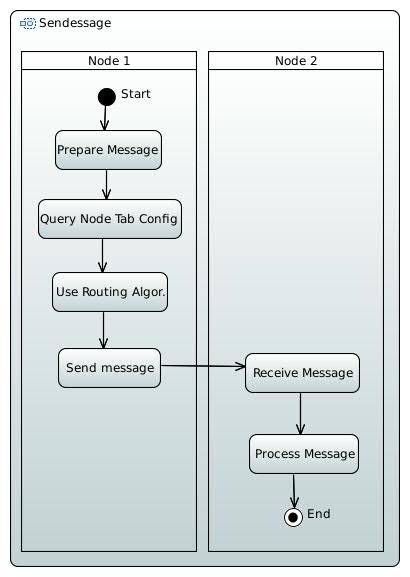
\includegraphics[scale=0.4]{images/Capitulo5/SendMessage.JPG}
  \caption{Diagrama de actividades del inicio de nodos}
  \label{fig:SendMessage}
\end{figure}


\vspace{1cm}
\noindent\rule{\textwidth}{2pt}

\textbf{\Large{Resúmen}}

En este capítulo se presentó la arquitectura propuesta, la cual 
sigue una filosofía de red distribuida que, como se estudio en
capítulos anteriores, brinda una mayor tolerancia a fallas.

La innovación de este trabajo puede ser observada en el diseño de
la arquitectura basado en modelos y orientado a objetos. Tanto la
arquitectura, como su protocolo de comunicación (CANae),
están basados en modelos, y utilizan el lenguaje de modelado SysML para su
modelado y documentación. 
